\documentclass{article}

\usepackage{graphicx}
\usepackage{tikz}
\usepackage{tikzsymbols}
\usetikzlibrary{calc,patterns,shapes.geometric}
\pagestyle{empty}
\usepackage[margin=0pt]{geometry}
\geometry{papersize={14in,12in}}

\def\centerarc[#1](#2)(#3:#4:#5){\draw[#1] ($(#2)+({#5*cos(#3)},{#5*sin(#3)})$) arc (#3:#4:#5);}

\begin{document}
	\begin{figure}
		\centering
		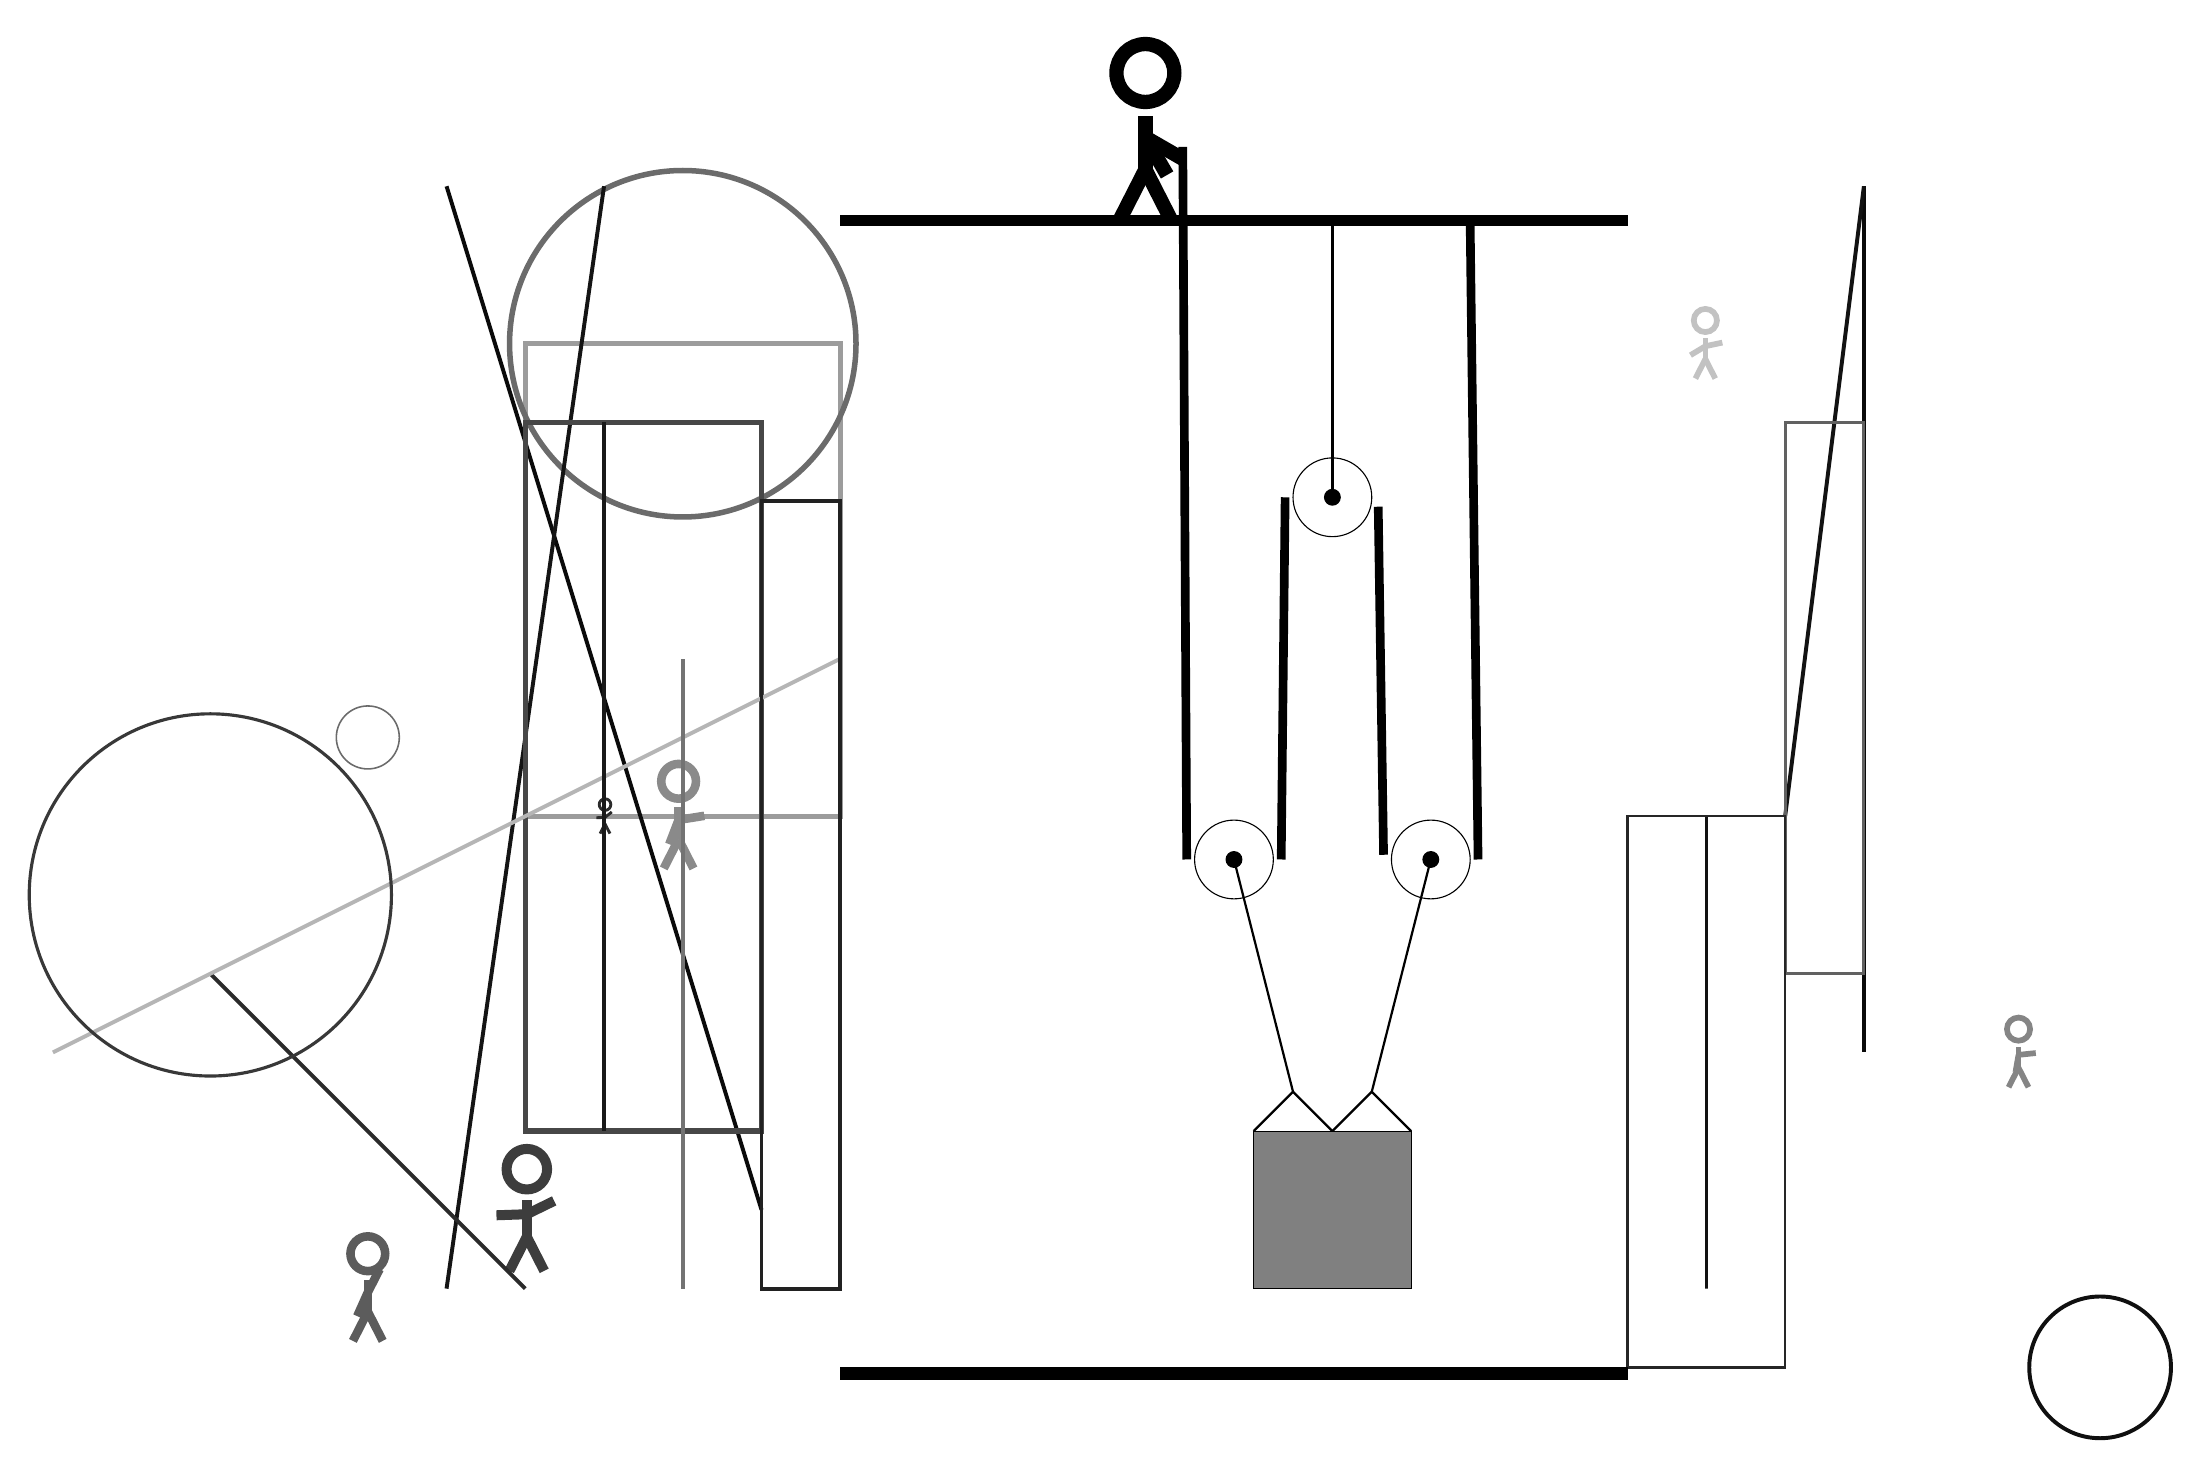
\begin{tikzpicture}
			%%%%% START %%%%%
			
			\draw[fill=black] (-4, 11.5) rectangle (6, 11.625);
			
			\draw (1, 3.45) circle (0.5);
			\draw[fill=black] (1, 3.45) circle (0.1);
			
			\draw (2.25, 8.05) circle (0.5);
			\draw[fill=black] (2.25, 8.05) circle (0.1);
			\draw[thick] (2.25, 8.05) -- (2.25, 11.5);
			
			\draw (3.5, 3.45) circle (0.5);
			\draw[fill=black] (3.5, 3.45) circle (0.1);
			
			\draw[thick] (3.5, 3.45) -- (2.75, 0.5);
			\draw[thick] (1, 3.45) -- (1.75, 0.5);
			\draw[thick]  (1.25, 0) -- (1.75, 0.5) -- (2.25, 0);
			\draw[thick]  (2.25, 0) -- (2.75, 0.5) -- (3.25, 0);
			\draw[fill=black!50] (1.25, 0) rectangle (3.25, -2);
			
			\draw[line width=1.1mm] (0.35, 12.5) --  (0.4, 3.45);
			\centerarc[line width=1.1mm](1, 3.45)(180:360:0.6);
			\draw[line width=1.1mm] (1.6, 3.45) -- (1.65, 8.05);
			\centerarc[line width=1.1mm](2.25, 8.05)(-20:180:0.6);
			\draw[line width=1.1mm](2.832, 7.93) -- (2.9, 3.51);
			\centerarc[line width=1.1mm](3.5, 3.45)(160:360:0.6);
			\draw[line width=1.1mm](4.1, 3.45) -- (4.0, 11.5);
			
			\draw[line width=0.6mm, color=black!39] (-4, 10) rectangle (-8, 4);
			
			\draw[line width=0.5mm, color=black!96](9, 12) -- (9, 1);
			\draw[line width=0.5mm, color=black!96](-5, -1) -- (-9, 12);
			\draw [line width=0.7mm, color=black!58](-6, 10) circle (2.2);
			
			\node[line width=0.5mm, color=black!76] at (-8, -1) {\Strichmaxerl[7][2][26]};
			
			\draw[line width=0.5mm, color=black!93](9, 12) -- (8, 4);
			\draw[line width=0.5mm, color=black!92](-9, -2) -- (-7, 12);
			\node[line width=0.4mm, color=black!46] at (-6, 4) {\Strichmaxerl[6][69][9]};
			\draw[line width=0.7mm, color=black!72] (-5, 9) rectangle (-8, 0);
			
			\node[line width=0.5mm, color=black!24] at (7, 10) {\Strichmaxerl[4][31][12]};
			
			\draw [line width=0.2mm, color=black!58](-10, 5) circle (0.4);
			\draw[line width=0.3mm, color=black!93] (7, -2) rectangle (7, 4);
			\node[line width=0.7mm, color=black!83] at (-7, 4) {\Strichmaxerl[2][2][39]};
			
			\node[line width=0.6mm, color=black!48] at (11, 1) {\Strichmaxerl[4][80][6]};
			\draw[line width=0.5mm, color=black!83](-8, -2) -- (-12, 2);
			\draw[line width=0.5mm, color=black!29](-4, 6) -- (-14, 1);
			\draw[line width=0.4mm, color=black!62] (8, 9) rectangle (9, 2);
			\draw [line width=0.3mm, color=black!61](-5, 3) circle (0.0);
			\draw[line width=0.3mm, color=black!85] (6, -3) rectangle (8, 4);
			\draw[line width=0.5mm, color=black!55](-6, -2) -- (-6, 6);
			\draw[line width=0.5mm, color=black!90](-7, 9) -- (-7, 0);
			\draw [line width=0.5mm, color=black!94](12, -3) circle (0.9);
			\draw [line width=0.4mm, color=black!78](-12, 3) circle (2.3);
			\draw[line width=0.5mm, color=black!87] (-4, -2) rectangle (-5, 8);
			\node[line width=0.5mm, color=black!64] at (-10, -2) {\Strichmaxerl[6][66][63]};
			
			
			\node at (-0.07, 12.7) {\Strichmaxerl[10][120][-30]};
			
			\draw[fill=black] (-4, -3) rectangle (6, -3.15);
			
			%%%%% END %%%%%
		\end{tikzpicture}
	\end{figure}	
\end{document}